\documentclass[11pt,a4paper]{article}
\usepackage[T1]{fontenc}
\usepackage[utf8]{inputenc}
\usepackage[margin=1in]{geometry}
\usepackage{amsmath,amsthm,mathtools}
\usepackage{newtxtext,newtxmath}
\usepackage[scaled=0.92]{inconsolata}
\usepackage{bm}
\usepackage{microtype}
\usepackage{booktabs,array,makecell}
\usepackage{graphicx}
\usepackage{xcolor}
\usepackage{enumitem}
\usepackage[font=small,labelfont=bf]{caption}
\usepackage{tikz}
\usetikzlibrary{arrows.meta,positioning,calc}
\usepackage[ruled,vlined,linesnumbered]{algorithm2e}
\usepackage{listings}
\usepackage[most]{tcolorbox}
\usepackage{placeins}

\definecolor{sone}{HTML}{2A78D6}
\definecolor{stwo}{HTML}{EB6834}
\definecolor{inktwo}{HTML}{52514E}
\definecolor{rule}{HTML}{C3C2B7}
\definecolor{wash}{HTML}{F4F7FB}
\usepackage[colorlinks=true,linkcolor=sone,urlcolor=sone,citecolor=sone,pdftitle={How gpedm\_py works},pdfsubject={Mathematical description of the Python port of GPEDM}]{hyperref}

\newcommand{\code}[1]{\texttt{\detokenize{#1}}}
\newcommand{\T}{^{\mathsf T}}
\newcommand{\R}{\mathbb{R}}
\newcommand{\obs}{\mathcal{O}}
\newcommand{\Sig}{\bm{\Sigma}}
\newcommand{\Siginv}{\bm{\Sigma}^{-1}}
\newcommand{\ve}{V_e}
\DeclareMathOperator{\tr}{tr}
\DeclareMathOperator{\sign}{sign}
\DeclareMathOperator{\clip}{clip}
\DeclareMathOperator{\diag}{diag}

\lstset{basicstyle=\ttfamily\small, columns=fullflexible, keepspaces=true, showstringspaces=false,
        frame=single, rulecolor=\color{rule}, backgroundcolor=\color{wash}, xleftmargin=4pt, xrightmargin=4pt,
        aboveskip=8pt, belowskip=8pt}

% a marked box for the places where the code does something a reader would not expect
\newtcolorbox{ascoded}[1][]{enhanced, breakable, colback=wash, colframe=wash, boxrule=0pt,
  borderline west={2pt}{0pt}{sone}, left=8pt, right=6pt, top=4pt, bottom=4pt, sharp corners,
  before skip=8pt, after skip=8pt, fontupper=\small, title={#1}, coltitle=black,
  fonttitle=\small\bfseries, attach title to upper={\ }}

\setlist{itemsep=2pt, topsep=4pt}
\setlength{\parskip}{4pt plus 1pt}
\setlength{\parindent}{0pt}
\numberwithin{equation}{section}

\begin{document}

\begin{center}
{\LARGE\bfseries How \code{gpedm_py} works}\\[6pt]
{\large Mathematical description of the Python port of GPEDM\\ used in the IceLab-EDM RespiCast forecast}\\[8pt]
{\small Describes \code{gpedm_py.py}, a port of GPEDM 0.0.0.9010, and the weekly forecast built on it, as of 14 October 2026}
\end{center}
\vspace{4pt}

\section{Overview}

\code{gpedm_py.py} fits a Gaussian process to a delay-embedded time series and predicts from it.
It ports, function by function, the three functions of the R package GPEDM~\cite{gpedm} that the
forecast calls: \code{makelags}, \code{fitGP} and \code{predict}. The method is Gaussian-process
empirical dynamic modelling~\cite{munch2017}, with the variable-step lags of~\cite{johnson2022} for
series that have gaps.

The calculation has four steps (Figure~\ref{fig:pipeline}). The series is turned into a regression
table whose predictors are earlier values of the series. Response and predictors are standardised.
The hyperparameters of a Gaussian process are set by maximising a log posterior with the Rprop
optimiser. The fitted process then gives a predictive mean and standard deviation for any new row
of predictors.

\begin{figure}[htbp]
\centering
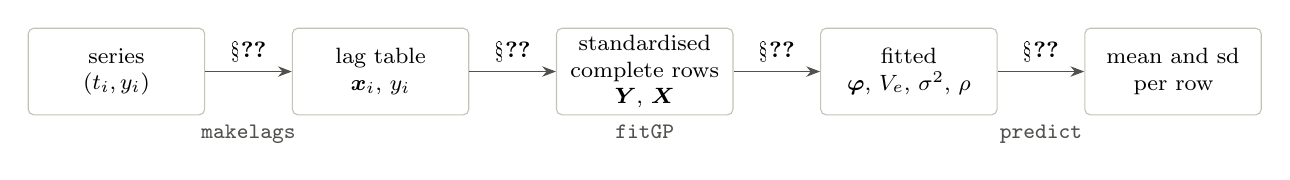
\begin{tikzpicture}[font=\footnotesize, node distance=11mm,
  box/.style={draw=rule, rounded corners=2pt, minimum height=11mm, text width=21mm, align=center, inner sep=2pt},
  arr/.style={-{Stealth[length=5pt]}, draw=inktwo}]
\node[box] (a) {series\\ $(t_i, y_i)$};
\node[box, right=of a] (b) {lag table\\ $\bm{x}_i$, $y_i$};
\node[box, right=of b] (c) {standardised complete rows\\ $\bm{Y}$, $\bm{X}$};
\node[box, right=of c] (d) {fitted\\ $\bm{\varphi}$, $\ve$, $\sigma^2$, $\rho$};
\node[box, right=of d] (e) {mean and sd\\ per row};
\draw[arr] (a) -- node[above]{\S\ref{sec:lags}} (b);
\draw[arr] (b) -- node[above]{\S\ref{sec:scaling}} (c);
\draw[arr] (c) -- node[above]{\S\ref{sec:fit}} (d);
\draw[arr] (d) -- node[above]{\S\ref{sec:predict}} (e);
\node[below=0.5mm of $(a)!0.5!(b)$, text=inktwo, yshift=-5mm] {\code{makelags}};
\node[below=0.5mm of $(b)!0.5!(d)$, text=inktwo, yshift=-5mm] {\code{fitGP}};
\node[below=0.5mm of $(d)!0.5!(e)$, text=inktwo, yshift=-5mm] {\code{predict}};
\end{tikzpicture}
\caption{The four steps and the function that performs each.}
\label{fig:pipeline}
\end{figure}

In code, a forecast of the next four time steps is three calls:
\begin{lstlisting}
lags = makelags(df, y="X", time="Time", E=E, tau=1, vtimestep=True)
fit  = fitGP(pd.concat([df, lags], axis=1), y="X", x=list(lags.columns), time="Time")
fore = makelags(df, y="X", time="Time", E=E, tau=1, vtimestep=True,
                forecast=True, Tdiff_fore=[1, 2, 3, 4])
pred = predict(fit, newdata=fore).outsampresults    # predmean, predfsd, predsd
\end{lstlisting}
That is how the RespiCast forecast used the port up to the round with origin date 14 October 2026.
From the round of 21 October 2026 it calls \code{makelags} no more: \code{gpedm_direct.py} builds one
table of fixed-step inputs per horizon and fits one Gaussian process to each
(Section~\ref{sec:direct}),
\begin{lstlisting}
for h in (1, 2, 3, 4):
    train, fore, xcols = direct_design(z, h, range(E), first_week, season=True, diff=True)
    fit  = fitGP(train, y="y", x=xcols, time="Time")
    pred = predict(fit, newdata=fore).outsampresults
\end{lstlisting}
Sections~\ref{sec:model} to~\ref{sec:predict} describe \code{fitGP} and \code{predict}, which both
forecasts use; Section~\ref{sec:respicast} describes the two forecasts.

\paragraph{Agreement with R.} On the 36 series of the RespiCast round with origin date 14 October 2026
the port and R~4.4.1 return identical lag tables, iteration counts and fitted parameters. Forecast
means agree to $4\times10^{-10}$ relative and forecast standard deviations to $1.1\times10^{-6}$
relative; that remainder is rounding in the matrix inverse of the worst-conditioned series.

\paragraph{Conventions.} Rows are numbered from 1 in this document and from 0 in the code. Bold
lower-case letters are vectors and bold capitals are matrices; $\circ$ is the elementwise product.
Appendix~\ref{app:names} maps every symbol to its name in the code.

\section{Lags: from a series to a regression table}
\label{sec:lags}

Let $y_1,\dots,y_n$ be the series, recorded at times $t_1<\dots<t_n$. Some values may be missing;
$\obs\subseteq\{1,\dots,n\}$ is the set of rows with an observed value. The embedding dimension
$E\ge1$ and the lag step $\tau\ge1$ are integers. \code{makelags} returns, for every row $i$, a
vector of predictors $\bm{x}_i$ built from earlier rows; row $i$ of the regression table is then
$(\bm{x}_i, y_i)$.

\subsection{Fixed step}
With \code{vtimestep=False} the lags are counted in rows:
\begin{equation}
\bm{x}_i = \bigl(y_{i-\tau},\; y_{i-2\tau},\; \dots,\; y_{i-E\tau}\bigr),
\end{equation}
with an entry missing when its index is below 1. A missing $y_j$ makes every row that uses it
incomplete, so one gap removes up to $E+1$ rows from the fit. The series must have $n>E\tau$ rows.

With \code{forecast=True} the function returns the $\tau$ rows that follow the series,
\begin{equation}
\bm{x}^{\mathrm f}_r = \bigl(y_{n-\tau+r},\; y_{n-2\tau+r},\; \dots,\; y_{n-E\tau+r}\bigr),
\qquad r=1,\dots,\tau,
\end{equation}
at times $t_n + r\,(t_n-t_{n-1})$.

\subsection{Variable step}
\label{sec:vts}
With \code{vtimestep=True} missing rows are skipped and the time that separates consecutive lags
becomes a predictor. For row $i>E\tau$ define the rows the lags are taken from by
\begin{equation}
\ell_0(i)=i,\qquad
\ell_k(i)=\max\bigl\{\,j\in\obs \;:\; j\le\min\bigl(i-k\tau,\;\ell_{k-1}(i)-\tau\bigr)\bigr\},
\qquad k=1,\dots,E .
\label{eq:lagrows}
\end{equation}
Lag $k$ is the latest observed row that lies at least $k\tau$ rows before row $i$ and at least
$\tau$ rows before lag $k-1$. The predictors are the $E$ lagged values followed by the $E$ time gaps,
\begin{equation}
\bm{x}_i=\bigl(y_{\ell_1(i)},\dots,y_{\ell_E(i)},\;\Delta_{i1},\dots,\Delta_{iE}\bigr),
\qquad \Delta_{ik}=t_{\ell_{k-1}(i)}-t_{\ell_k(i)} ,
\label{eq:vtsrow}
\end{equation}
so the table has $d=2E$ predictor columns, named \code{X_1}, \dots, \code{X_E}, \code{Tdiff_1},
\dots, \code{Tdiff_E} for a variable called \code{X}. For $\tau=1$, definition~\eqref{eq:lagrows}
reduces to: lag $k$ is the $k$-th most recent observed row before row $i$.

Three details follow from~\eqref{eq:lagrows}.
\begin{itemize}
\item The first $E\tau$ rows get no lags at all, whatever the data.
\item If the set in~\eqref{eq:lagrows} is empty for some $k$, lag $k$ and all deeper lags are missing.
\item The bounds count \emph{rows}, while the gaps $\Delta_{ik}$ are differences of \emph{times}.
The two coincide only when the rows are equally spaced.
\end{itemize}
A row whose own value $y_i$ is missing still receives lags; it is dropped later, when the fit
keeps complete rows only.

\subsection{Forecast rows}
With \code{forecast=True} and steps ahead $h_1,\dots,h_H$ (\code{Tdiff_fore}), rows $n+1,\dots,n+H$
are appended at times $t_{n+m}=t_n+h_m$, with unknown value, and~\eqref{eq:lagrows} is applied to
them with $\obs$ unchanged. Only these $H$ rows are returned. For $\tau=1$ every forecast row
has the same lagged values, the last $E$ observed values of the series, and the same gaps
$\Delta_2,\dots,\Delta_E$. The rows differ only in the first gap,
\begin{equation}
\Delta_{n+m,1}=t_n+h_m-t_{\ell_1}, \qquad\text{which is } h_m \text{ when the last row is observed.}
\label{eq:foregap}
\end{equation}
The forecast horizon therefore enters the model through one number, the column \code{Tdiff_1}.
If \code{Tdiff_fore} is not given it defaults to the single step $\tau\min_i(t_{i+1}-t_i)$.

\subsection{Several variables, several populations, long gaps}
With $v$ variables, a row counts as observed when all $v$ are present; each variable contributes
its $E$ lagged values at the same rows $\ell_k(i)$, and the $E$ gaps follow, so $d=E(v+1)$. With a
population column the construction runs separately within each population. \code{Tdiff_max} sets
every gap larger than it to missing, which removes those rows from the fit.

\subsection{Example}
Take $n=10$ rows at times $t_i=i$, with $y_4$, $y_7$ and $y_8$ missing, $E=2$ and $\tau=1$.
Figure~\ref{fig:lags} shows the lags of row 9 and of a forecast row; Table~\ref{tab:lags} lists
the whole table as \code{makelags} returns it.

\begin{figure}[htbp]
\centering
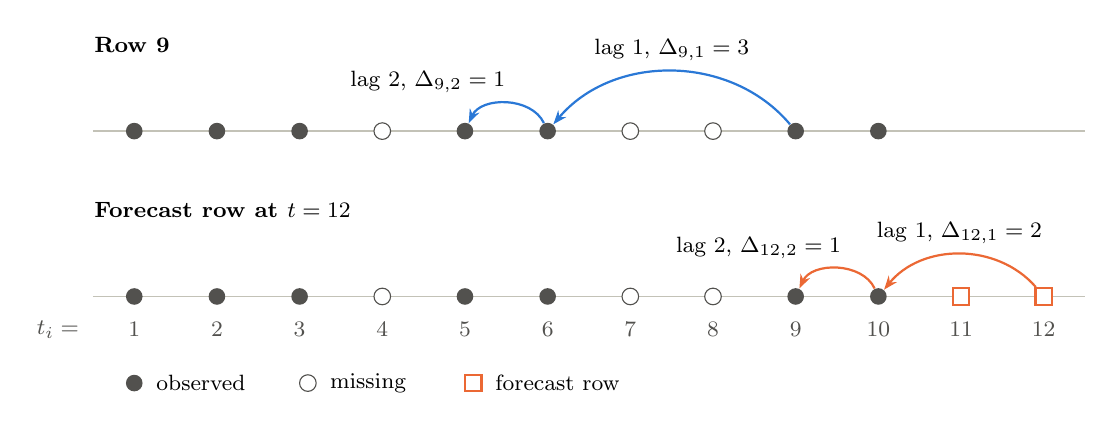
\begin{tikzpicture}[x=10.5mm, y=10mm, font=\footnotesize,
  obsdot/.style={circle, fill=inktwo, inner sep=0pt, minimum size=6pt},
  misdot/.style={circle, draw=inktwo, fill=white, inner sep=0pt, minimum size=6pt},
  foredot/.style={rectangle, draw=stwo, fill=white, line width=0.8pt, inner sep=0pt, minimum size=6pt},
  lag/.style={-{Stealth[length=5pt]}, line width=0.8pt}]
% an ordinary row
\begin{scope}
\node[anchor=west] at (0.4,1.1) {\textbf{Row 9}};
\draw[rule, line width=0.6pt] (0.5,0) -- (12.5,0);
\foreach \i in {1,2,3,5,6,9,10} {\node[obsdot] (a\i) at (\i,0) {};}
\foreach \i in {4,7,8} {\node[misdot] (a\i) at (\i,0) {};}
\draw[lag, sone] (a9) to[bend right=50] node[above, text=black]{lag 1, $\Delta_{9,1}=3$} (a6);
\draw[lag, sone] (a6) to[bend right=65] (a5);
\node at (4.55,0.62) {lag 2, $\Delta_{9,2}=1$};
\end{scope}
% a forecast row
\begin{scope}[yshift=-21mm]
\node[anchor=west] at (0.4,1.1) {\textbf{Forecast row at $t=12$}};
\draw[rule, line width=0.6pt] (0.5,0) -- (12.5,0);
\foreach \i in {1,2,3,5,6,9,10} {\node[obsdot] (b\i) at (\i,0) {};}
\foreach \i in {4,7,8} {\node[misdot] (b\i) at (\i,0) {};}
\foreach \i in {11,12} {\node[foredot] (b\i) at (\i,0) {};}
\draw[lag, stwo] (b12) to[bend right=50] node[above, text=black]{lag 1, $\Delta_{12,1}=2$} (b10);
\draw[lag, stwo] (b10) to[bend right=65] (b9);
\node at (8.55,0.62) {lag 2, $\Delta_{12,2}=1$};
\foreach \i in {1,...,12} {\node[text=inktwo] at (\i,-0.42) {\i};}
\node[text=inktwo, anchor=east] at (0.45,-0.42) {$t_i=$};
\node[obsdot] at (1,-1.1) {}; \node[anchor=west] at (1.15,-1.1) {observed};
\node[misdot] at (3.1,-1.1) {}; \node[anchor=west] at (3.25,-1.1) {missing};
\node[foredot] at (5.1,-1.1) {}; \node[anchor=west] at (5.25,-1.1) {forecast row};
\end{scope}
\end{tikzpicture}
\caption{Variable-step lags for $E=2$, $\tau=1$; an arrow points from a row to the row its lag is
taken from. Row 9 skips the two missing rows: its first lag is row 6, three time steps back, and its
second lag is row 5. The forecast row at $t=12$ takes the last two observed rows; only its first
gap differs from that of the forecast row at $t=11$.}
\label{fig:lags}
\end{figure}

\begin{table}[htbp]
\centering\small
\begin{tabular}{@{}rlllccl@{}}
\toprule
$i$ & $y_i$ & \code{y_1} & \code{y_2} & \code{Tdiff_1} & \code{Tdiff_2} & use \\
\midrule
1 & $y_1$ & -- & -- & -- & -- & no lags ($i\le E\tau$) \\
2 & $y_2$ & -- & -- & -- & -- & no lags ($i\le E\tau$) \\
3 & $y_3$ & $y_2$ & $y_1$ & 1 & 1 & fitted \\
4 & missing & $y_3$ & $y_2$ & 1 & 1 & dropped, no response \\
5 & $y_5$ & $y_3$ & $y_2$ & 2 & 1 & fitted \\
6 & $y_6$ & $y_5$ & $y_3$ & 1 & 2 & fitted \\
7 & missing & $y_6$ & $y_5$ & 1 & 1 & dropped, no response \\
8 & missing & $y_6$ & $y_5$ & 2 & 1 & dropped, no response \\
9 & $y_9$ & $y_6$ & $y_5$ & 3 & 1 & fitted \\
10 & $y_{10}$ & $y_9$ & $y_6$ & 1 & 3 & fitted \\
\midrule
11 & to predict & $y_{10}$ & $y_9$ & 1 & 1 & forecast row, $h=1$ \\
12 & to predict & $y_{10}$ & $y_9$ & 2 & 1 & forecast row, $h=2$ \\
\bottomrule
\end{tabular}
\caption{The lag table of the example. Five of the ten rows can be fitted. With fixed-step lags
only row 3 would be complete.}
\label{tab:lags}
\end{table}

\section{The model}
\label{sec:model}

\subsection{Standardising and selecting rows}
\label{sec:scaling}
\code{fitGP} receives the response column and $d$ predictor columns. With the default
\code{scaling="global"} each column is centred and scaled by its own mean and standard deviation,
\begin{equation}
\tilde y_i=\frac{y_i-m_y}{s_y},\qquad \tilde x_{ik}=\frac{x_{ik}-m_k}{s_k},
\label{eq:scale}
\end{equation}
where a column's mean and standard deviation (denominator: count minus one) are taken over all rows
in which that column is present. \code{scaling="local"} does the same within each population, and
\code{scaling="none"} uses the columns as given.

The fit keeps the \emph{complete rows}: those with a response and all $d$ predictors. Let there
be $N$ of them, collected in $\bm{Y}\in\R^N$ and $\bm{X}\in\R^{N\times d}$; from here on
$i,j=1,\dots,N$ index these rows and $\bm{x}_i$ is row $i$ of $\bm{X}$.

A constant column has $s_k=0$, so~\eqref{eq:scale} gives $0/0$ for every row and no row is
complete. This is what happens to the gap columns of~\eqref{eq:vtsrow} when a series has no gap at
all: every $\Delta_{ik}$ equals the sampling interval. \code{gpedm_py} raises an error in that case.

\subsection{Prior over functions and likelihood}
The standardised response is modelled as a smooth function of the predictors plus independent noise,
\begin{equation}
Y_i=f(\bm{x}_i)+\varepsilon_i,\qquad \varepsilon_i\sim\mathcal N(0,\ve),\qquad f\sim\mathcal{GP}(0,c),
\end{equation}
with the squared-exponential covariance function, one coefficient per input,
\begin{equation}
c(\bm{x},\bm{x}')=\sigma^2\exp\Bigl(-\sum_{k=1}^{d}\varphi_k\,(x_k-x'_k)^2\Bigr)\,r,
\qquad
r=\begin{cases}1 & \text{same population}\\ \rho & \text{different populations.}\end{cases}
\label{eq:cov}
\end{equation}
The mean function is zero because the response has been centred. The coefficient $\varphi_k$ is an
inverse squared length scale: $\exp(-\varphi_k u^2)=\exp\bigl(-u^2/2\ell_k^2\bigr)$ with
$\ell_k=(2\varphi_k)^{-1/2}$, measured in standard deviations of input $k$. As $\varphi_k\to0$ the
function stops depending on input $k$, which is how the fit selects among the lags.

Write $\bm{C}$ for the $N\times N$ matrix with entries $C_{ij}=c(\bm{x}_i,\bm{x}_j)$ and
\begin{equation}
\Sig=\bm{C}+\ve\,\bm{I}.
\end{equation}
Then $\bm{Y}\sim\mathcal N(\bm 0,\Sig)$, and the log likelihood of the hyperparameters
$\bm\theta=(\varphi_1,\dots,\varphi_d,\ve,\sigma^2,\rho)$ is, up to a constant,
\begin{equation}
L(\bm\theta)=-\tfrac12\,\bm{Y}\T\Siginv\bm{Y}-\tfrac12\log\det\Sig .
\label{eq:loglik}
\end{equation}
The code factorises $\Sig=\bm{R}\T\bm{R}$ with $\bm{R}$ upper triangular, forms $\Siginv$
explicitly from the factor (LAPACK \code{dpotrf} and \code{dpotri}, as R does), and uses
\begin{equation}
\bm{a}=\Siginv\bm{Y},\qquad \bm{Y}\T\Siginv\bm{Y}=\bm{Y}\T\bm{a},\qquad
\tfrac12\log\det\Sig=\sum_{i=1}^{N}\log R_{ii}.
\end{equation}

\subsection{Priors}
The hyperparameters have independent priors:
\begin{align}
\pi(\varphi_k)&\propto\exp\Bigl(-\frac{\varphi_k^2}{2\lambda}\Bigr),\quad \varphi_k>0,
\qquad \lambda=\bigl(2^{\,m-1}\bigr)^2\,\frac{\pi}{2}, \label{eq:priorphi}\\
\ve/V_{\max}&\sim\mathrm{Beta}(2,2),\qquad \sigma^2/\sigma^2_{\max}\sim\mathrm{Beta}(2,2),\qquad
\rho\sim\mathrm{Beta}(2,2),
\end{align}
with $V_{\max}=\sigma^2_{\max}=4.9999$. The half-normal prior~\eqref{eq:priorphi} has mean
$\sqrt{2\lambda/\pi}=2^{\,m-1}$, where $m$ is the argument \code{modeprior} (default 1, so
$\lambda=\pi/2$ and the prior mean of every $\varphi_k$ is 1). Up to a constant,
\begin{equation}
\log\pi(\bm\theta)=-\frac{1}{2\lambda}\sum_{k=1}^{d}\varphi_k^2
+\log\frac{\ve}{V_{\max}}+\log\Bigl(1-\frac{\ve}{V_{\max}}\Bigr)
+\log\frac{\sigma^2}{\sigma^2_{\max}}+\log\Bigl(1-\frac{\sigma^2}{\sigma^2_{\max}}\Bigr)
+\log\rho+\log(1-\rho).
\label{eq:logprior}
\end{equation}

\subsection{Unconstrained parameters}
The optimiser works on a vector $\bm{p}\in\R^{d+3}$ without constraints (Table~\ref{tab:pars}):
\begin{equation}
\varphi_k=e^{p_k},\qquad
\theta=\theta_{\min}+\frac{\theta_{\max}-\theta_{\min}}{1+e^{-p}}\quad\text{for }\theta\in\{\ve,\sigma^2,\rho\},
\label{eq:transform}
\end{equation}
with derivatives
\begin{equation}
\frac{d\varphi_k}{dp_k}=\varphi_k,\qquad
\frac{d\theta}{dp}=(\theta-\theta_{\min})\Bigl(1-\frac{\theta-\theta_{\min}}{\theta_{\max}-\theta_{\min}}\Bigr).
\label{eq:dtransform}
\end{equation}
The prior~\eqref{eq:logprior} is a density in $\bm\theta$ and no Jacobian term is added for the
change of variables, so the fit targets the posterior mode in $\bm\theta$, not in $\bm{p}$.

\begin{table}[htbp]
\centering\small
\begin{tabular}{@{}llllll@{}}
\toprule
 & meaning & range & prior & start & in $\bm{p}$ \\
\midrule
$\varphi_k$ & inverse squared length scale of input $k$ & $(0,\infty)$ & half-normal, mean $2^{m-1}$ & 0.1 & $\log\varphi_k$ \\
$\ve$ & noise variance & $(10^{-4},\,4.9999)$ & $\mathrm{Beta}(2,2)$ on $\ve/4.9999$ & 0.001 & logistic \\
$\sigma^2$ & variance of $f$ & $(10^{-4},\,4.9999)$ & $\mathrm{Beta}(2,2)$ on $\sigma^2/4.9999$ & 0.999 & logistic \\
$\rho$ & correlation between populations & $(10^{-4},\,1)$ & $\mathrm{Beta}(2,2)$ & 0.5 & logistic \\
\bottomrule
\end{tabular}
\caption{The $d+3$ hyperparameters. Variances are on the standardised scale, where the response
has variance 1. With a single population $\rho$ is not estimated: it is held at 0.5 and has no
effect.}
\label{tab:pars}
\end{table}

\section{Fitting}
\label{sec:fit}

\subsection{Objective and gradient}
The fit minimises the negative log posterior
\begin{equation}
F(\bm{p})=-\Bigl[L\bigl(\bm\theta(\bm{p})\bigr)+\log\pi\bigl(\bm\theta(\bm{p})\bigr)\Bigr],
\label{eq:F}
\end{equation}
returned as \code{nllpost}; the fit statistic \code{ln_post} is $-F$ at the final point. For any
hyperparameter $\theta$ the derivative of~\eqref{eq:loglik} is~\cite[eq.~5.9]{rw2006}
\begin{equation}
\frac{\partial L}{\partial\theta}=\tr\Bigl(\bm{Q}\,\frac{\partial\Sig}{\partial\theta}\Bigr)
=\sum_{i,j}Q_{ij}\,\frac{\partial\Sigma_{ij}}{\partial\theta},
\qquad \bm{Q}=\tfrac12\bigl(\bm{a}\bm{a}\T-\Siginv\bigr),
\label{eq:dL}
\end{equation}
and from~\eqref{eq:cov}, with $D^{(k)}_{ij}=(X_{ik}-X_{jk})^2$ and $S_{ij}=1$ when rows $i$ and $j$
belong to the same population and 0 otherwise,
\begin{equation}
\frac{\partial\Sig}{\partial\varphi_k}=-\bm{D}^{(k)}\circ\bm{C},\qquad
\frac{\partial\Sig}{\partial\ve}=\bm{I},\qquad
\frac{\partial\Sig}{\partial\sigma^2}=\frac{\bm{C}}{\sigma^2},\qquad
\frac{\partial\Sig}{\partial\rho}=\frac{\bm{C}\circ(\bm{1}\bm{1}\T-\bm{S})}{\rho}.
\label{eq:dSigma}
\end{equation}
The prior~\eqref{eq:logprior} contributes
\begin{equation}
\frac{\partial\log\pi}{\partial\varphi_k}=-\frac{\varphi_k}{\lambda},\qquad
\frac{\partial\log\pi}{\partial\ve}=\frac{1}{\ve}-\frac{1}{V_{\max}-\ve},\qquad
\frac{\partial\log\pi}{\partial\rho}=\frac1\rho-\frac1{1-\rho},
\end{equation}
and the same form as for $\ve$ holds for $\sigma^2$. The gradient that \code{getlikegrad} returns,
and that drives the optimiser, is
\begin{equation}
g_k=-\Bigl(\gamma_k\,\frac{\partial L}{\partial\theta_k}+\frac{\partial\log\pi}{\partial\theta_k}\Bigr)
\frac{d\theta_k}{dp_k},
\qquad
\gamma_k=\begin{cases}\tfrac12 & \text{for } \varphi_1,\dots,\varphi_d\\[2pt] 1 & \text{for } \ve,\ \sigma^2,\ \rho .\end{cases}
\label{eq:g}
\end{equation}

\begin{ascoded}[The factor $\gamma_k=\tfrac12$.]
The exact gradient of~\eqref{eq:F} has $\gamma_k=1$ for every parameter. GPEDM multiplies the
likelihood part of the $\varphi$ entries by a further one half, and the port does the same so that
its results match R. Finite differences of $F$ confirm it: for every $\varphi_k$ whose gradient is
clear of rounding noise the ratio of the coded to the numerical likelihood gradient is 0.50, and it
is 1.00 for $\ve$ and $\sigma^2$ (\code{gpedm_py_validation/check_gradient.py}).
Section~\ref{sec:effective} states what this does to the fit.
\end{ascoded}

\subsection{The optimiser}
\code{fmingrad_Rprop} is Rprop~\cite{riedmiller1993} in the variant without backtracking, often
written Rprop$^-$~\cite{igel2003}. Each parameter has its own step size. A step moves every
parameter against the sign of its gradient entry by its step size; the size of the gradient is
never used. A step size grows by a factor 1.2 when its gradient entry kept its sign and halves when
the sign flipped (Algorithm~\ref{alg:rprop}).

\begin{algorithm}[htbp]
\DontPrintSemicolon
\KwIn{start $\bm{p}$ from Table~\ref{tab:pars}; data $\bm{Y}$, $\bm{X}$}
$\bm\delta\gets0.1\cdot\bm1$;\quad $t\gets0$;\quad $q\gets10$;\quad $(F,\bm{g})\gets$ objective~\eqref{eq:F} and gradient~\eqref{eq:g} at $\bm{p}$\;
\While{$\lVert\bm{g}\rVert_2>10^{-4}$ \textbf{and} $t<200$ \textbf{and} $q>10^{-7}$}{
  $\bm{p}'\gets\bm{p}-\sign(\bm{g})\circ\bm\delta$\;
  $(F',\bm{g}')\gets$ objective and gradient at $\bm{p}'$\;
  $q\gets\lvert F'/F-1\rvert$\;
  \For{$k=1,\dots,d+3$}{
    $\delta_k\gets\clip\bigl(\eta_k\,\delta_k,\;10^{-6},\;50\bigr)$,\quad
    $\eta_k=1.2$ if $g_kg'_k>0$,\ \ $0.5$ if $g_kg'_k<0$,\ \ $1$ if $g_kg'_k=0$\;
  }
  $(\bm{p},F,\bm{g})\gets(\bm{p}',F',\bm{g}')$;\quad $t\gets t+1$\;
}
\KwOut{$\bm{p}$, and with it $\bm\theta$, $\Sig$, $\Siginv$ and $\bm{a}$ at the final point}
\caption{\code{fmingrad_Rprop}}
\label{alg:rprop}
\end{algorithm}

\subsection{What the optimiser maximises}
\label{sec:effective}
\begin{enumerate}[label=(\roman*)]
\item \textbf{The effective prior on $\bm\varphi$.} Because only signs are used, multiplying
gradient entries by positive constants does not change the path. By~\eqref{eq:g},
$\bm{g}=\bm{\Gamma}\,\nabla\tilde F$ with $\bm\Gamma=\diag(\tfrac12,\dots,\tfrac12,1,1,1)$ and
\begin{equation}
\tilde F(\bm{p})=-\Bigl[L+2\log\pi(\bm\varphi)+\log\pi(\ve)+\log\pi(\sigma^2)+\log\pi(\rho)\Bigr].
\end{equation}
The iterates are therefore those of Rprop applied to $\tilde F$: the fit is the posterior mode
with the half-normal prior on each $\varphi_k$ counted twice, that is with variance parameter
$\lambda/2$ in place of $\lambda$. The identity was checked numerically at the fitted point of the
two series of Section~\ref{sec:respicast}. The reported \code{nllpost} is still $F$, and
the stopping rule is evaluated on $F$ and on $\bm{g}$.
\item \textbf{Stopping.} The loop ends when the gradient norm falls below $10^{-4}$, when the
relative change $q$ of the objective falls below $10^{-7}$, or after 200 iterations. $q$ is a
ratio of successive values of $F$, which has no fixed sign, so $q$ is large whenever $F$ passes
near zero (Figure~\ref{fig:trace}, iterations 14 and 15).
\item \textbf{No step is rejected.} There is no line search: $F$ may rise from one iteration to
the next, and the final point is the last iterate, not the best one. In the fit of
Section~\ref{sec:respicast} $F$ rises at iterations 12, 27, 28 and 38, the last one.
\item \textbf{Determinism.} The start is fixed and nothing is random, so a fit is a function of
the data. The path depends on the data only through gradient signs, which is why the port
reproduces the parameters of R exactly although its arithmetic differs in the last digit.
\item \textbf{Inputs switched off.} A step size can reach 50 on the log scale, so $p_k$ can run
far below zero in a few iterations. Below about $-745$, $\varphi_k=e^{p_k}$ is exactly 0 in double
precision and input $k$ is removed from the covariance.
\item \textbf{Fixed parameters.} A parameter fixed through \code{fixedpars} or \code{rhofixed}
has its likelihood derivative set to zero, but its prior derivative stays in $\bm{g}$ and so in the
gradient norm of the stopping rule. The value used in $\Sig$ is always the fixed one.
\end{enumerate}

\section{Prediction}
\label{sec:predict}

All predictions are computed on the standardised scale from the quantities stored at the end of
the fit, $\bm{C}$, $\Sig$, $\Siginv$ and $\bm{a}=\Siginv\bm{Y}$, and then transformed back
(Section~\ref{sec:back}). Three numbers are returned per row: the mean, the standard deviation of
the function $f$ alone (\code{predfsd}) and the standard deviation of a new observation
(\code{predsd}), which adds the noise variance $\ve$.

\subsection{Fitted values}
For the rows used in the fit, the posterior mean and covariance of $f$ are
\begin{equation}
\hat{\bm f}=\bm{C}\bm{a},\qquad \operatorname{Cov}(\bm f\mid\bm Y)=\bm{C}-\bm{C}\Siginv\bm{C},
\end{equation}
and \code{insampresults} holds $\hat f_i$, $\sqrt{v_i}$ and $\sqrt{v_i+\ve}$ with $v_i$ the
$i$-th diagonal entry of the covariance.

\subsection{New inputs}
A new row of predictors is standardised with the means and standard deviations of the training
data~\eqref{eq:scale}. With $\bm{c}_*=\bigl(c(\bm{x}_*,\bm{x}_1),\dots,c(\bm{x}_*,\bm{x}_N)\bigr)\T$,
\begin{equation}
\mu_*=\bm{c}_*\T\bm{a},\qquad v_*=\sigma^2-\bm{c}_*\T\Siginv\bm{c}_* ,
\label{eq:pred}
\end{equation}
and the row gets mean $\mu_*$, \code{predfsd} $\sqrt{v_*}$ and \code{predsd} $\sqrt{v_*+\ve}$. A new
row with a missing predictor gets missing predictions. Far from all training rows
$\bm{c}_*\to\bm0$, so $\mu_*\to0$ and $v_*\to\sigma^2$: the prediction returns to the prior, which
on the original scale is the mean of the series with standard deviation $s_y\sqrt{\sigma^2+\ve}$.

\subsection{Leave-one-out}
\code{predictmethod="loo"} predicts each fitted row $i$ from the others. With exclusion radius
$r$ (\code{exclradius}), the rows left out are those of the same population within $r$ positions
of $i$ in the fitted data; let $K$ be the remaining rows. Then
\begin{equation}
\mu_{-i}=\bm{C}_{iK}\,\Sig_{KK}^{-1}\,\bm{Y}_K,\qquad
v_{-i}=\sigma^2-\bm{C}_{iK}\,\Sig_{KK}^{-1}\,\bm{C}_{Ki},
\end{equation}
computed with one matrix inverse per row. For $r=0$ these have the closed
form~\cite[Sec.~5.4.2]{rw2006}
\begin{equation}
\mu_{-i}=Y_i-\frac{a_i}{[\Siginv]_{ii}},\qquad v_{-i}+\ve=\frac{1}{[\Siginv]_{ii}},
\label{eq:looclosed}
\end{equation}
which the loop reproduces to better than $10^{-12}$ on the series of Section~\ref{sec:respicast}. The
fit statistic \code{lnL_LOO} is the leave-one-out log predictive density from~\eqref{eq:looclosed},
without its constant:
\begin{equation}
\texttt{lnL\_LOO}=\sum_{i=1}^{N}\Bigl(\tfrac12\log[\Siginv]_{ii}-\tfrac12\,\frac{a_i^2}{[\Siginv]_{ii}}\Bigr).
\end{equation}
The hyperparameters are not refitted when rows are left out.

\subsection{Leave-time-out}
\code{predictmethod="lto"} leaves out whole time points, in all populations at once. Let
$\tau_1,\dots,\tau_T$ be the distinct times of the fitted rows in order of first appearance. For
time point $u$ the training set $K$ is every row whose time is not among
$\tau_{u-r},\dots,\tau_{u+r}$, and all rows at $\tau_u$ are predicted from $K$ with the formulas
above. The radius counts positions in the list of time points, not units of time.

\subsection{Sequential}
\code{predictmethod="sequential"} predicts each time point from the earlier ones, with the fitted
hyperparameters. Starting from $\bm m^{(1)}=\bm0$ and $\bm S^{(1)}=\bm C$, and with $I_u$ the rows
at time point $\tau_u$, the update for $u=1,\dots,T-1$ is
\begin{align}
\bm K_u&=\bigl(\bm S^{(u)}_{I_uI_u}+\ve\bm I\bigr)^{-1},\\
\bm m^{(u+1)}&=\bm m^{(u)}+\bm S^{(u)}_{\,\cdot\, I_u}\bm K_u\bigl(\bm Y_{I_u}-\bm m^{(u)}_{I_u}\bigr),\qquad
\bm S^{(u+1)}=\bm S^{(u)}-\bm S^{(u)}_{\,\cdot\, I_u}\bm K_u\bm S^{(u)}_{I_u\,\cdot} .
\end{align}
A row $j\in I_u$ is predicted from the data of time points $\tau_1,\dots,\tau_{u-1}$: its mean is
$m^{(u)}_j$ and, for $u\ge2$, its \code{predsd} is $\sqrt{\lvert S^{(u)}_{jj}\rvert+\ve}$
(Section~\ref{sec:notes} has the case $u=1$). \code{predfsd} is $\sqrt{\texttt{predsd}^2-\ve}$.

\subsection{Back-transformation and fit statistics}
\label{sec:back}
With global scaling a standardised mean $\mu$ and variance $v$ become
\begin{equation}
\texttt{predmean}=m_y+s_y\,\mu,\qquad \texttt{predfsd}=s_y\sqrt{v},\qquad \texttt{predsd}=s_y\sqrt{v+\ve},
\end{equation}
and with local scaling the population's own $m_y$ and $s_y$ are used. \code{insampfitstats} reports,
besides \code{ln_post}, \code{ln_prior} and \code{lnL_LOO}: $R^2=1-\sum(y_i-\hat y_i)^2/\sum(y_i-\bar y)^2$
and the root mean squared error of the fitted values on the original scale; the effective number
of parameters $\texttt{df}=\tr(\bm C\Siginv)$; $\texttt{SS}=\bm Y\T\Siginv\bm Y$; and
$\texttt{logdet}=\tfrac12\log\det\Sig$.

\section{Use in the RespiCast forecast}
\label{sec:respicast}

\code{respi_edm.run_analysis} forecasts each country and target separately. Two models have been
submitted. Up to the round with origin date 14 October 2026 it was one Gaussian process on
variable-step lags whose four horizons differ only in a time-gap input
(Section~\ref{sec:old}). From the round of 21 October 2026 it is one Gaussian process per horizon on
the log scale, with the time of year as input (Sections~\ref{sec:direct} and~\ref{sec:direct-numbers}),
chosen on a replay of 85 past rounds (Section~\ref{sec:replay}).

\subsection{The forecast from 21 October 2026}
\label{sec:direct}
The code is \code{gpedm_direct.forecast}, called by \code{respi_edm.run_analysis} with its default
\code{method="direct"}.

\paragraph{Which series.} The weekly values of one country are laid out by date, $x_1,\dots,x_n$,
from its first to its last observation; a week without a report is missing, and no week is blanked.
Let $k$ be the number of weeks from the last observation $x_n$ to the newest week of the round, the
week before the target week of horizon 1. The series is forecast if
\begin{itemize}
\item $k\le1$ (\code{respi_edm.MAX_WEEKS_MISSING}), judged by the latest date in the data, not by the
first row: the hub lists the rows of the UK nations and of Swiss ILI oldest first, and the test on the
first row skipped those series up to 14 October 2026 although their newest week was present;
\item at least 30 weeks are observed, and every horizon has at least 30 complete training rows.
\end{itemize}
Skipped series are named in a printed message.

\paragraph{Scale.} The model works with
\begin{equation}
z_i=\log(x_i+c),\qquad c=\max\bigl(1,\ \bar x/10\bigr),
\label{eq:logscale}
\end{equation}
where $\bar x$ is the mean of the observed values and $c$ is rounded to six significant digits. An
offset in proportion to the level of the series keeps a zero, or a very small value, in a series of
large values from becoming an extreme point on the log scale. For Belgian ARI, $c=94.09$.

\paragraph{Embedding dimension.} $E\le8$ is chosen by the false-nearest-neighbour test, as before
(the random generator is seeded with 42, because the mutual-information step jitters its input).

\paragraph{One regression per horizon.} The forecast for the hub's horizon $h=1,\dots,4$ lies
$H=k+h$ weeks after the last observation. Its training rows are the weeks $s$ with
\begin{equation}
\bm x^{(H)}_s=\bigl(z_s,\ \tilde z_{s-1},\ \dots,\ \tilde z_{s-E+1},\ \sin\theta_{s+H},\ \cos\theta_{s+H}\bigr),
\qquad
y^{(H)}_s=z_{s+H}-z_s ,
\label{eq:directrow}
\end{equation}
where $\theta_t=2\pi\,(\text{day of the year of the last day of week }t-1)/365.25$ is the time of year of
the target week, and $\tilde z$ is $z$ with missing weeks filled by linear interpolation between
observed weeks, which for a lag lie at or before week $s$. A row is complete when $z_s$ and $z_{s+H}$
are observed and $s\ge E$. The $d=E+2$ inputs are all on a fixed step, so no column is constant and
no week has to be blanked (compare Section~\ref{sec:scaling}). \code{fitGP} is called with one
population, global scaling and the default priors and start, once for each $H$, so each horizon has
its own hyperparameters.

\paragraph{Forecast.} The forecast row is the last week, $\bm x^{(H)}_n$. \code{predict}~\eqref{eq:pred}
gives the mean $\mu_H$ and the standard deviation $\sigma_H$ (\code{predsd}, which includes $\ve$) of the
change $z_{n+H}-z_n$. The forecast distribution is
\begin{equation}
z_{n+H}\sim\mathcal N\bigl(z_n+\mu_H,\ \sigma_H^2\bigr),\qquad
\hat x_{q}=\max\Bigl(0,\ \exp\bigl(z_n+\mu_H+\Phi^{-1}(q)\,\sigma_H\bigr)-c\Bigr),
\label{eq:directq}
\end{equation}
a log-normal shifted by $c$ and cut at zero, with $\Phi$ the standard normal distribution function. The
submission holds, for each horizon, the 23 hub quantiles $\hat x_q$ and the median $\hat x_{0.5}$.

\begin{ascoded}[As coded.]
\code{direct_design} returns every week $s=1,\dots,n-H$ as a row; \code{fitGP} drops the incomplete
ones (Section~\ref{sec:scaling}). A lag longer than the series stays missing, so such an $E$ gives no
forecast rather than an error. A series with $k=1$ is fitted with $H=2,\dots,5$ and its four
forecasts are submitted as the hub's horizons 1 to 4. The table that \code{run_analysis} returns holds,
per horizon, $k$ (\code{weeks_missing}), $E$, the transform \code{log:}$c$, $z_n+\mu_H$, $\sigma_H$ and
the median.
\end{ascoded}

\subsection{One forecast in numbers}
\label{sec:direct-numbers}
Belgium ARI on the round with origin date 14 October 2026 (the same data as in
Section~\ref{sec:old-numbers}): $n=224$ weeks from 26 June 2022, none missing, $\bar x=940.9$,
$c=94.09$, $E=3$, last value $x_n=1071.3$. Table~\ref{tab:direct} lists the four fits.

\begin{table}[htbp]
\centering\small
\begin{tabular}{@{}lrrrr@{}}
\toprule
horizon $H$ & 1 & 2 & 3 & 4 \\
\midrule
complete rows $N$ & 221 & 220 & 219 & 218 \\
optimiser iterations & 58 & 68 & 69 & 74 \\
length scale $\ell$ of $z_s$ & 1.75 & 1.44 & 1.75 & 1.81 \\
\phantom{length scale $\ell$ of }$z_{s-1}$ & 2.15 & 4.33 & 2.69 & 2.53 \\
\phantom{length scale $\ell$ of }$z_{s-2}$ & -- & 9.18 & 3.07 & 2.97 \\
\phantom{length scale $\ell$ of }$\sin\theta$ & 0.58 & 0.50 & 0.49 & 0.49 \\
\phantom{length scale $\ell$ of }$\cos\theta$ & 1.04 & 0.78 & 0.79 & 0.86 \\
noise variance $\ve$ & 0.541 & 0.307 & 0.194 & 0.149 \\
variance of $f$, $\sigma^2$ & 2.83 & 2.41 & 2.32 & 1.87 \\
s.d.\ of the change $z_{s+H}-z_s$, $s_y$ & 0.184 & 0.244 & 0.313 & 0.370 \\
\midrule
forecast change $\mu_H$ & $+0.043$ & $+0.024$ & $-0.031$ & $-0.076$ \\
forecast s.d.\ $\sigma_H$ & 0.148 & 0.151 & 0.167 & 0.175 \\
median $\hat x_{0.5}$ & 1122.6 & 1099.2 & 1035.7 & 985.8 \\
95\% interval & 816--1532 & 794--1509 & 720--1473 & 672--1429 \\
\bottomrule
\end{tabular}
\caption{The four fits of the forecast for Belgium ARI. Length scales are in standard deviations of
the input (--: $\varphi=0$, the input is switched off). The time of year has the shortest length scales:
the fits learn above all how the weekly change depends on the season. The forecast standard
deviation is a small fraction of $s_y$, the spread of the change over the whole series.}
\label{tab:direct}
\end{table}

In Slovakia ($c=145.55$, $E=3$, last value 1282.5) the medians are 1359.7, 1553.4, 1619.4 and
1495.3, where the previous model gave 1257.8 at every horizon (Figure~\ref{fig:direct}).

\begin{figure}[htbp]
\centering
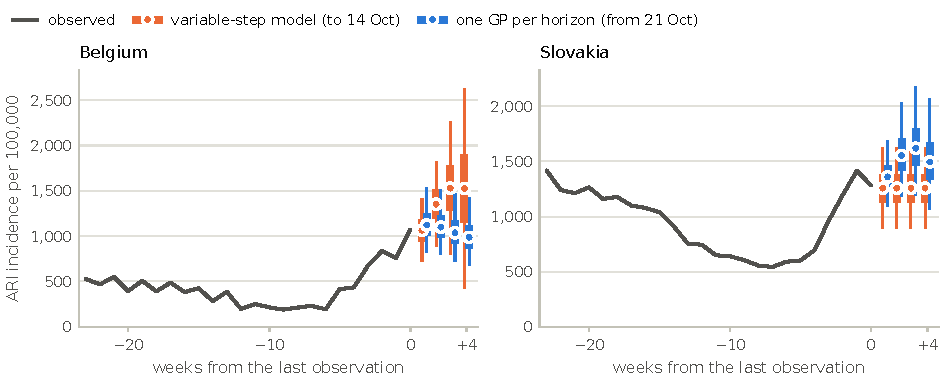
\includegraphics[width=\textwidth]{figures/fig_direct.pdf}
\caption{The two ARI series of Figure~\ref{fig:forecast}, forecast on the same data by the model
submitted up to 14 October 2026 (orange) and by the one submitted from 21 October 2026 (blue): median,
50\% and 95\% intervals.}
\label{fig:direct}
\end{figure}

\subsection{Why this model: a replay of 85 rounds}
\label{sec:replay}
Each model variant was run on every past round from origin date 16 October 2024 to 7 October 2026,
on the hub data as published on the Friday before the origin date, and scored like the hub scores
the submitted models: the weighted interval score (WIS) against the values published later, turned
into a rank score $(\text{WIS}_{\text{worst}}-\text{WIS})/(\text{WIS}_{\text{worst}}-\text{WIS}_{\text{best}})$
among the other models of the hub for the same country, target and week (about 11 models). A score of 1
is the best model on that forecast. The mean is over 8,844 forecasts of 43 series; the intervals are
95\% block-bootstrap intervals over origin dates of the difference from the submitted model. The code
is in \code{gpedm_method_tests/}.

\begin{table}[htbp]
\centering\small
\begin{tabular}{@{}lcc@{}}
\toprule
variant & rank score & difference (95\% interval) \\
\midrule
hub quantile baseline & 0.697 & \\
model submitted up to 14 October (variable step, incidence scale) & 0.690 & 0 \\
\quad + time of year as input & 0.724 & $+0.034$ ($0.021$ to $0.049$) \\
\quad + log scale, $c=1$ & 0.739 & $+0.049$ ($0.031$ to $0.067$) \\
\quad + both & 0.776 & $+0.086$ ($0.069$ to $0.107$) \\
one Gaussian process per horizon & 0.699 & $+0.009$ ($-0.009$ to $0.029$) \\
\quad + log scale, $c=1$ & 0.772 & $+0.082$ ($0.067$ to $0.098$) \\
\quad + log scale + time of year & 0.795 & $+0.105$ ($0.080$ to $0.130$) \\
\quad + the same, change as response & 0.802 & $+0.112$ ($0.087$ to $0.137$) \\
\quad + offset $c=\max(1,\bar x/10)$: \textbf{submitted from 21 October} & \textbf{0.807} & $+0.117$ ($0.092$ to $0.144$) \\
hub ensemble & 0.807 & \\
\bottomrule
\end{tabular}
\caption{Mean rank score of each variant over the same 8,844 forecasts. The offset $c=\bar x/10$ adds
$0.005$ ($0.003$ to $0.008$) to $c=1$; it mostly repairs Luxembourg ILI, where single zeros in a series
of large values become outliers with $c=1$.}
\label{tab:replay}
\end{table}

Tried and not adopted, with the difference from the submitted model:
\begin{itemize}
\item \textbf{Two embedding dimensions mixed}, one short (1 to 8 weeks) and one long (26 to 78 weeks), as
the average of the two forecasts' quantiles: every pair with a short $E$ of 2 to 6 scores 0.793 to 0.799,
the best pair (3 and 53) $-0.009$ ($-0.021$ to $0.004$). A year-long $E$ alone scores 0.73.
\item \textbf{Neighbouring countries as inputs} (six forms: their mean level, each neighbour, all other
countries, their growth, their level relative to the country's own): $-0.005$ to $-0.001$.
\item \textbf{The exact gradient of $\varphi$} instead of GPEDM's halved one (Section~\ref{sec:notes}):
no change.
\item \textbf{One Gaussian process for all countries}, with the country as population: $+0.013$ ($0.006$
to $0.020$) over the same model fitted to each country alone, on every second round and with $E=3$ and
the last 208 weeks; not yet tried with the offset $c=\bar x/10$.
\end{itemize}

\paragraph{Series behind by one week.} Forecasting a series from a last value that is $k$ weeks old
costs accuracy. Table~\ref{tab:stale} compares the series the run forecast up to 14 October with those it
skipped. The model stays level with the hub ensemble on the skipped series, but they are harder, so
submitting them lowers the model's mean rank score from 0.807 to 0.800 ($-0.0075$, $-0.011$ to
$-0.003$) while adding a fifth more forecasts. The run allows $k\le1$ from 21 October 2026.

\begin{table}[htbp]
\centering\small
\begin{tabular}{@{}lrrcc@{}}
\toprule
series on the origin date & series-dates & \makecell[r]{ranked\\forecasts} & \makecell{rank\\score} & \makecell{hub\\ensemble} \\
\midrule
newest week in the first row (submitted to 14 October) & 2,399 & 8,844 & 0.807 & 0.797 \\
newest week present, rows listed oldest first & 169 & 283 & 0.752 & 0.724 \\
last value one week old ($k=1$) & 444 & 1,445 & 0.763 & 0.762 \\
last value two weeks old ($k=2$, not submitted) & 149 & 418 & 0.747 & 0.709 \\
\bottomrule
\end{tabular}
\caption{Rank score of the submitted model by how current the series was on the origin date, with the
hub ensemble's rank score on the same forecasts. The first three rows are what the run submits from
21 October 2026.}
\label{tab:stale}
\end{table}

\subsection{The model submitted up to 14 October 2026}
\label{sec:old}
\code{respi_edm.run_analysis(method="vt")} still computes it (with \code{backend="r"} or
\code{"python"}).
\begin{enumerate}
\item The weekly incidence values are laid out as a vector $y_1,\dots,y_n$ with time $t_i=i-1$;
weeks without a report are missing.
\item The 21st value is set to missing (index 20 in the code). Without at least one gap every
\code{Tdiff} column is constant and no row survives (Section~\ref{sec:scaling}).
\item The embedding dimension $E\le8$ is chosen by a false-nearest-neighbour test. That test is run
at a lag picked by mutual information, while the lags below are built with $\tau=1$.
\item Variable-step lags with $\tau=1$ give $d=2E$ predictors~\eqref{eq:vtsrow}. One population,
global scaling, default priors and start.
\item Forecast rows for $h=1,2,3,4$ weeks ahead~\eqref{eq:foregap} are predicted
with~\eqref{eq:pred}, giving $\mu_h=\texttt{predmean}$ and $\sigma_h=\texttt{predsd}$.
\item The submission holds, for each horizon, the median $\max(0,\mu_h)$ and the 23 hub quantiles
$\max\bigl(0,\;\mu_h+\Phi^{-1}(q)\,\sigma_h\bigr)$, with $\Phi$ the standard normal distribution
function.
\end{enumerate}
Only series whose first row is the newest week are forecast. The data step of this path lays the
weeks out on a year $\times$ week-number grid. It fails on a series that contains an ISO week 53 (the
first is the week ending 3 January 2027), and in a series that never reports some week numbers it
moves the summer gap to the turn of the year. The model of Section~\ref{sec:direct} lays the weeks out
by date and has neither problem.

\subsubsection{One fit in numbers}
\label{sec:old-numbers}
The numbers of this section, the next and Section~\ref{sec:direct-numbers} are produced by
\code{gpedm_py_docs/make_numbers.py}.

Belgium, acute respiratory infections (ARI), origin date 14 October 2026: $n=224$ weeks, one gap
(the blanked week), $E=3$, so $d=6$ and $N=220$ complete rows. The optimiser stops after 38
iterations on the relative-change rule, with $F=-73.27$ and a gradient norm still at
$1.1\times10^{-2}$ (Figure~\ref{fig:trace}). Table~\ref{tab:belgium} lists the result.

\begin{table}[htbp]
\centering\small
\begin{tabular}{@{}lccl@{\hspace{2.5em}}lc@{}}
\toprule
input & $\varphi_k$ & $\ell_k$ & & quantity & value \\
\cmidrule(r){1-3}\cmidrule(l){5-6}
\code{X_1} (last value) & $2.5\times10^{-2}$ & 4.5 & & noise variance $\ve$ & 0.159 \\
\code{X_2} & $7.1\times10^{-4}$ & 26.5 & & variance of $f$, $\sigma^2$ & 3.66 \\
\code{X_3} & $2.1\times10^{-3}$ & 15.4 & & $m_y$, $s_y$ (per 100,000) & 940.4,\ 440.7 \\
\code{Tdiff_1} & $4.1\times10^{-4}$ & 35.0 & & in-sample $R^2$ & 0.848 \\
\code{Tdiff_2} & $1.5\times10^{-3}$ & 18.5 & & effective parameters \code{df} & 6.35 \\
\code{Tdiff_3} & $6.5\times10^{-195}$ & -- & & \code{lnL_LOO} & 88.1 \\
\bottomrule
\end{tabular}
\caption{Fitted hyperparameters for Belgium ARI. Length scales $\ell_k=(2\varphi_k)^{-1/2}$ are in
standard deviations of the input. All are several standard deviations long, so the fitted function
varies slowly over the range of the data; the third gap is switched off.}
\label{tab:belgium}
\end{table}

\begin{figure}[htbp]
\centering
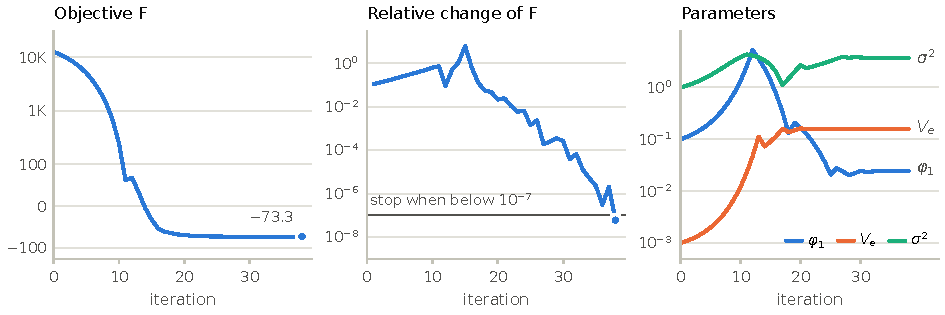
\includegraphics[width=\textwidth]{figures/fig_trace.pdf}
\caption{The optimiser on Belgium ARI. Left: the objective, on a symmetric log scale, falls from
12,497 to $-73.3$. Centre: its relative change, the quantity that ends the loop; the peak at
iterations 14 and 15 is $F$ passing through zero. Right: three of the eight free parameters on their
natural scale.}
\label{fig:trace}
\end{figure}

\subsubsection{What the time gap does to the four horizons}
\label{sec:horizons}
The four forecast rows are identical except for the first gap, $\Delta_1=h$~\eqref{eq:foregap}.
Let $\varphi_\Delta$ be the coefficient of the column \code{Tdiff_1}, $s_\Delta$ its standard
deviation, and $\Delta_j$ its value in fitted row $j$. Because the covariance~\eqref{eq:cov} is a
product over inputs, the covariance of the horizon-$h$ row with fitted row $j$ is the
horizon-1 covariance times a factor that depends only on the gap of row $j$:
\begin{equation}
c_{*j}(h)=c_{*j}(1)\,\kappa_h(\Delta_j),\qquad
\kappa_h(\Delta)=\exp\Bigl(-\varphi_\Delta\,\frac{(h-\Delta)^2-(1-\Delta)^2}{s_\Delta^2}\Bigr).
\label{eq:kappa}
\end{equation}
The standardised forecast mean~\eqref{eq:pred} is then a sum over the gap values present in the
fitted rows,
\begin{equation}
\mu(h)=\sum_{\Delta}\kappa_h(\Delta)\,T_\Delta,\qquad
T_\Delta=\sum_{j:\,\Delta_j=\Delta}c_{*j}(1)\,a_j ,
\label{eq:decomp}
\end{equation}
where $T_\Delta$ is what the rows with gap $\Delta$ contribute to the one-week forecast.
Three regimes follow.
\begin{itemize}
\item \textbf{$\varphi_\Delta=0$.} Then $\kappa_h\equiv1$ and the forecast, mean and standard
deviation, is the same at every horizon. In 20 of the 36 series of the round the fitted
$\varphi_\Delta$ is below $10^{-89}$ and this is what the submission contains.
\item \textbf{$\varphi_\Delta>0$.} Rows with gap 1 are down-weighted by
$\kappa_h(1)=\exp\bigl(-\varphi_\Delta(h-1)^2/s_\Delta^2\bigr)$. The scale $s_\Delta$ is small
because nearly every fitted gap equals 1. When the blanked week is the only gap, the column holds
$M-1$ ones and a single two over the $M$ rows where it is defined, its variance is exactly $1/M$,
and
\begin{equation}
\kappa_h(1)=\exp\bigl(-\varphi_\Delta\,M\,(h-1)^2\bigr):
\end{equation}
a forecast row at horizon $h$ lies $(h-1)\sqrt{M}$ standard deviations from all but one of the
fitted rows. For $M=221$ that is 15, 30 and 45 standard deviations for $h=2,3,4$.
\item \textbf{$\varphi_\Delta M\gg1$.} Then $\kappa_h(1)\approx0$ for $h\ge2$. The two-week
forecast rests on the rows with gap 2 alone. For $h\ge3$ no fitted row is close, $\mu(h)\to0$ and
$v(h)\to\sigma^2$: the forecast is the mean of the series with the prior standard deviation
$s_y\sqrt{\sigma^2+\ve}$.
\end{itemize}

Table~\ref{tab:decomp} evaluates~\eqref{eq:decomp} for Belgium, where
$\varphi_\Delta M=4.08\times10^{-4}\times221=0.090$; the sum reproduces the forecasts of the code
to all printed digits. The single row that follows the blanked week contributes $+3.77$ to a
one-week mean of $0.28$, against $-3.49$ from the other 219 rows together, and its weight relative
to theirs grows with the horizon. The forecasts for weeks 2 to 4 hinge on that one row, and so on
which week was blanked. In Slovakia $\varphi_\Delta=9\times10^{-282}$ and all four forecasts coincide
(Figure~\ref{fig:forecast}).

\begin{table}[htbp]
\centering\small
\begin{tabular}{@{}lrrrrrr@{}}
\toprule
 & rows & $T_\Delta$ & $\kappa_1$ & $\kappa_2$ & $\kappa_3$ & $\kappa_4$ \\
\midrule
fitted rows with gap $\Delta=1$ & 219 & $-3.494$ & 1 & 0.914 & 0.697 & 0.444 \\
fitted row with gap $\Delta=2$ & 1 & $+3.773$ & 1 & 1.094 & 1 & 0.763 \\
\midrule
standardised mean $\mu(h)$ & & & 0.279 & 0.936 & 1.336 & 1.326 \\
\code{predmean} $=m_y+s_y\,\mu(h)$ & & & 1063.4 & 1352.9 & 1529.4 & 1525.0 \\
\code{predsd} & & & 177.2 & 238.8 & 372.8 & 562.4 \\
\bottomrule
\end{tabular}
\caption{The decomposition~\eqref{eq:decomp} for Belgium ARI. For comparison, the prior standard
deviation $s_y\sqrt{\sigma^2+\ve}$ is 861.6 and the last observed value is 1071.3.}
\label{tab:decomp}
\end{table}

\begin{figure}[htbp]
\centering
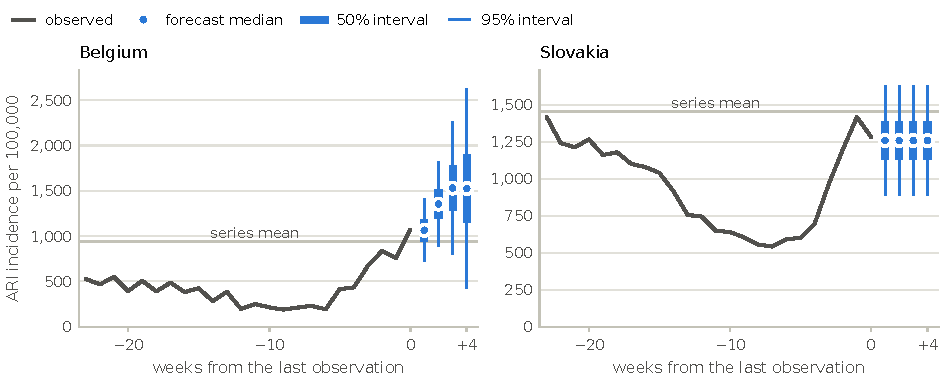
\includegraphics[width=\textwidth]{figures/fig_forecast.pdf}
\caption{Forecasts of the round with origin date 14 October 2026 for two ARI series, each with the
blanked week as its only gap. In Belgium the fit keeps the time gap
($\varphi_\Delta=4.1\times10^{-4}$) and the four horizons differ. In Slovakia the fit switches it
off and the four forecasts are the same number with the same interval.}
\label{fig:forecast}
\end{figure}

\FloatBarrier
\section{Where the port follows R, and where it does not}
\label{sec:notes}

The port reproduces the following behaviour of GPEDM on purpose. All but the last are marked
\code{NOTE} in the source.
\begin{itemize}
\item The likelihood gradient of the $\varphi_k$ carries the factor one half~\eqref{eq:g}.
\item The prior gradient of a fixed parameter stays in $\bm g$ (Section~\ref{sec:effective}, vi).
\item \code{makelags(vtimestep=True)} returns its rows grouped by population, in order of first
appearance. They line up with the data only if the data are sorted the same way.
\item The default \code{Tdiff_fore} is computed from the first population and reused for the others.
\item The exclusion radius of leave-one-out and leave-time-out counts rows and positions, not time.
\item In sequential prediction the first time point is reported with $\sigma^2+\ve$ where the
other rows carry a standard deviation, so that entry is a variance.
\item The lower bound of $\rho$ is 0 when the start value $\rho_0$ is transformed and $10^{-4}$ in
the likelihood, so with several populations the optimiser starts from
$10^{-4}+(1-10^{-4})\,\rho_0$, not from $\rho_0$.
\end{itemize}

The port differs from R in two respects.
\begin{itemize}
\item \textbf{No complete rows.} R fits zero rows without an error and its \code{predict} returns
missing values. \code{gpedm_py} raises an error that names the constant columns.
\item \textbf{Rounding.} R standardises the training data with \code{scale()} and new inputs with
\code{mean()} and \code{sd()}, and links another linear-algebra library. Results differ in the last
digits, amplified by the condition number of $\Sig$: at most $1.1\times10^{-6}$ relative in the 36
series compared, for a matrix with condition number $2.7\times10^{6}$.
\end{itemize}

Not ported: data augmentation (\code{augment}, \code{augdata}), \code{linprior}, \code{rhomatrix},
lags generated inside \code{fitGP} through its \code{E} and \code{tau} arguments,
\code{returnGPgrad}, the per-population $R^2$ tables, and the fisheries and iterated-forecast
functions.

\appendix
\section{Symbols and their names in the code}
\label{app:names}

\begin{center}\small
\begin{tabular}{@{}lll@{}}
\toprule
symbol & in \code{gpedm_py.py} & where \\
\midrule
$y_i$, $t_i$ & the \code{y} and \code{time} columns of \code{data} & \code{makelags}, \code{fitGP} \\
$\obs$ & \code{nm} & \code{makelags} \\
$\ell_{k-1}(i)$, $\ell_k(i)$ & \code{prev}, \code{new} & \code{makelags} \\
$\Delta_{ik}$ & columns \code{Tdiff_1}, \dots, \code{Tdiff_E} & output of \code{makelags} \\
$h_1,\dots,h_H$ & \code{Tdiff_fore} & \code{makelags} \\
$m_y$, $s_y$, $m_k$, $s_k$ & \code{ymeans}, \code{ysds}, \code{xmeans}, \code{xsds} & \code{fit.scaling} \\
$\bm Y$, $\bm X$ & \code{Y}, \code{X} & \code{fit.inputs} \\
$\bm\theta$ & \code{pars}: \code{phi1}, \dots, \code{ve}, \code{sigma2}, \code{rho} & \code{fit.pars} \\
$\bm p$ & \code{parst} & \code{fit.parst} \\
$\bm C$, $\Sig$, $\Siginv$ & \code{Cd}, \code{Sigma}, \code{iKVs} & \code{fit.covm} \\
$\bm R$, $\bm a$, $\bm Q$, $\bm D^{(k)}$ & \code{L}, \code{a}, \code{Q}, \code{D[k]} & \code{getlikegrad} \\
$\lambda$, $m$ & \code{lam_phi}, \code{modeprior} & \code{getpriors} \\
$F$, $\bm g$ & \code{nllpost}, \code{grad} & \code{getlikegrad}, \code{fit} \\
$\bm\delta$, $q$, $t$ & \code{delta}, \code{df}, \code{it} & \code{fmingrad_Rprop} \\
$\bm c_*$ & \code{Cs} & \code{predict} \\
$m_y+s_y\mu$, $s_y\sqrt{v}$, $s_y\sqrt{v+\ve}$ & \code{predmean}, \code{predfsd}, \code{predsd} & result tables \\
\midrule
\multicolumn{3}{@{}l}{\emph{the forecast from 21 October 2026} (Section~\ref{sec:direct})}\\
$c$ & the number in the transform name \code{log:}$c$ & \code{gpedm_direct.log_transform} \\
$z_i$ & \code{z} & \code{direct_forecast} \\
$k$, $H=k+h$ & \code{weeks_missing}, \code{horizons} & \code{forecast}, \code{direct_forecast} \\
$\bm x^{(H)}_s$, $y^{(H)}_s$ & columns \code{L0}, \dots, \code{L}$E{-}1$, \code{sea_sin}, \code{sea_cos}; \code{y} & \code{direct_design} \\
$z_n+\mu_H$, $\sigma_H$ & \code{Forecast.mean}, \code{Forecast.sd} & \code{gpedm_direct.forecast} \\
$\hat x_q$ & \code{Forecast.quantiles} & \code{gpedm_direct.quantiles} \\
\bottomrule
\end{tabular}
\end{center}

\begin{thebibliography}{9}\small
\bibitem{gpedm} S.~B. Munch and T.~L. Rogers. \emph{GPEDM: Gaussian Process regression for Empirical
Dynamic Modeling}. R package, version 0.0.0.9010. \url{https://tanyalrogers.github.io/GPEDM}
\bibitem{munch2017} S.~B. Munch, V. Poynor and J.~L. Arriaza. Circumventing structural uncertainty:
a Bayesian perspective on nonlinear forecasting for ecology. \emph{Ecological Complexity} 32
(2017), 134--143.
\bibitem{johnson2022} B. Johnson and S.~B. Munch. An empirical dynamic modeling framework for missing
or irregular samples. \emph{Ecological Modelling} 468 (2022).
\bibitem{rw2006} C.~E. Rasmussen and C.~K.~I. Williams. \emph{Gaussian Processes for Machine
Learning}. MIT Press, 2006.
\bibitem{riedmiller1993} M. Riedmiller and H. Braun. A direct adaptive method for faster
backpropagation learning: the RPROP algorithm. \emph{IEEE International Conference on Neural
Networks} (1993), 586--591.
\bibitem{igel2003} C. Igel and M. H\"usken. Empirical evaluation of the improved Rprop learning
algorithms. \emph{Neurocomputing} 50 (2003), 105--123.
\end{thebibliography}

\end{document}
